% LaTeX template for ENGR1000J-S2 Summer 2025 Final Project Report
\documentclass{engr1000j-s2}

% Main content
\begin{document}
  \thispagestyle{firstpage}
  
\includegraphics[height=0.8in]{figures/headlogo.png}
  \\ \textbf{\Large ENGR1000J Introduction to Engineering, Summer 2025}\\[0.5em]
  \textbf{{\Large \today}}\\[0em]

  \begin{center}

    \begin{minipage}{0.45\textwidth}
      
\includegraphics[height=0.8in]{figures/team logo.png}
    \end{minipage}\hfill
    \begin{minipage}{0.45\textwidth}
      \textbf{\Large Group 0: TC team}
    \end{minipage}\\[0.2em]
  \end{center}

  \noindent
  {\color{gray!30}\rule{\textwidth}{0.1pt}}

  {\Huge Project Title}

  {
\includegraphics[height=3in]{figures/preface_picture.png}}

  \hspace{1em}

  % Team members
  { 
  \Large 
  \setlength{\parskip}{5pt}
  \setlength{\baselineskip}{0pt}
  Team Member${}^{1}$ (\begin{CJK}
    {UTF8}{gbsn} 中文名
  \end{CJK}), \textit{\underline {email@address}}

  Zeyi Chen${}^{1}$ (\begin{CJK}
    {UTF8}{gbsn} 陈泽奕
  \end{CJK}),
  $\textit{\underline{\href{mailto:marzich_44@sjtu.edu.cn}{marzich\_44@sjtu.edu.cn}}
  }$

  Xinchang Wang${}^{1}$ (\begin{CJK}
    {UTF8}{gbsn} 王欣畅
  \end{CJK}),
  $\textit{\underline{\href{mailto:wang_xinchang@sjtu.edu.cn}{wang\_xinchang@sjtu.edu.cn}}
  }$

  Different Institute Member ${}^{2}$, \textit{\underline {email@address}}

  }

  \newpage
  \pagestyle{mystyle}
  % Abstract
  \section*{Abstract}
  \addcontentsline{toc}{section}{Abstract}
  This section includes information for those readers who will not read the entire document. Although this section appears first in the document, it is usually written last. It is one-paragraph long (not an introduction) and complete in itself (no reference numbers). It should indicate the general engineering background of your project and state the objectives. The design methodology, measurement techniques, observed facts, key understandings and conclusions must be stated in summary form. It should include a description of the project background, the project aim, the major tasks undertaken, the measurement techniques employed, key observations and physical understanding, conclusion and the significance of your findings. Word count is 200-400. 

  \hspace{1em}

  % Acknowledgments
  \section*{Acknowledgments}
  \addcontentsline{toc}{section}{Acknowledgments}
  Thank all parties who assisted this project, such as TAs, instructors, companies, and teammates.
  
  % Table of Contents
  \newpage
  \tableofcontents
  \thispagestyle{mystyle}
  \newpage

  % Main sections
  \section{Introduction}
  This section gives the reader a flavor of the work or project presented: the context
  of the work, the objectives, scope. In another word, the problem, the need, and
  the solution. Normally it begins with more general background, then gradually narrows
  down to a particular problem. After clearly identify the problem, what is needed
  will be liberated followed by a solution (brief summary of what your prototype
  can offer). The main goal of this section is to establish the significance of
  your project--why is it needed. (page limit 2 pages)

  Background is where you set the context for your work. You need to place your
  work in a context beyond the immediate engineering application. Current societal
  topics are a good place to start: security, energy, sustainability, productivity,
  etc. Spend some time discussing the broader engineering issues, then gradually
  narrow the discussion down to the technical side of your project. Background can
  include reasonable technical discussions on some fundamental theories related to
  your project. Please avoid your own personal opinion and keep all the
  discussions objective.

  Proper citation is always required per academic ethic and HC. List and number all
  references at the end of the report. Reference citations in the text should be
  in numerical order. [e.g., \citep{brandis2016nonequi}.].

  \hspace{1em}
  
  \textbf{Statements}
  \begin{itemize}
    \item Problem: clearly and concisely sums up what is the problem.\\

    \item Need/s: clearly and concisely sums up what is/are needed.\\

    \item Solution/s: clearly and concisely sums up the solution your project offers.
  \end{itemize}

  \hspace{1em}

  \section{Project Management}

  This section describes how your team managed this project. It should include a
  simple Gantt Chart, material budget, personnel information and contribution,
  and risk assessment. The tasks stated in the Gantt Chart correspond to the needs/solutions
  of this project.

  A Gantt chart provides concise but accurate information on the expected timetable
  for the project. The time for completion of each task should correspond
  exactly to the tasks previously described. Keep your Gantt Charts simple; as
  this graphic is intended for external audience, do not include too many tasks or
  descriptions of each task.

  Budget: State the proposed costs and budget of the project. Also include information
  on how you intend to manage the budget. One common way of showing the budget
  is according to the tasks as in Table \ref{tab:budget}.

  In building a set-up or prototype, material costs are typically accounted for in
  a bill of materials (BOM). This typically takes the form of the example shown
  below in Table \ref{tab:bill_of_materials}. State the costs of the project in an
  itemized form. Use a table, and make sure you list the total and any relevant sources
  for your purchases. If the purchasing link list is too long to fit in the main
  report body, you may include them as an appendix or a supplementary session.

  \begin{figure}[!ht]
    \centering
    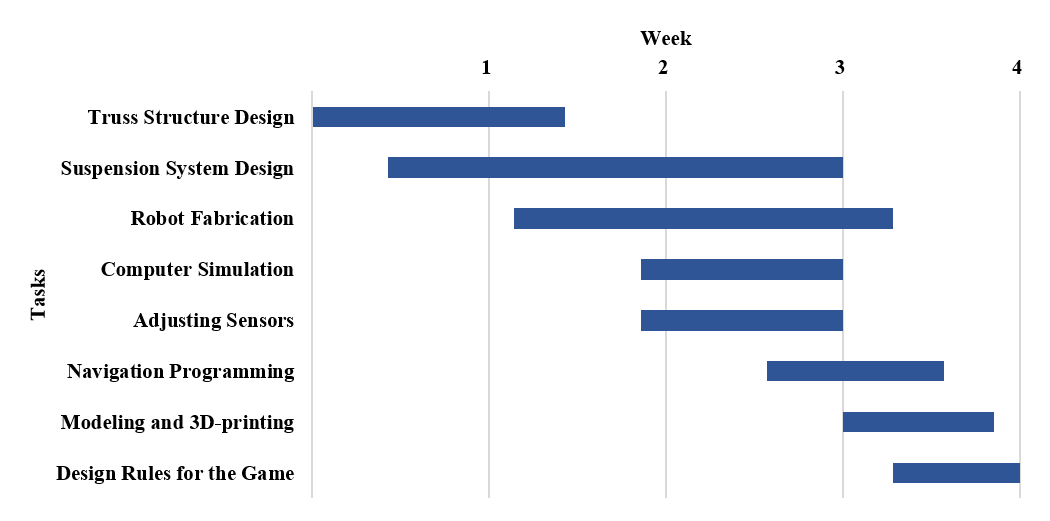
\includegraphics[width=0.8\textwidth]{figures/gantt_chart.png}
    \caption{\quad \textbf{Gantt chart for the project.}}
    \label{fig:gantt_chart}
  \end{figure}

  \begin{table}[h]
    \centering
    \caption{\quad \textbf{Project estimated budget}}
    \begin{tabular}{
      p{0.15\textwidth} 
      >{\centering\arraybackslash}p{0.45\textwidth} 
      >{\centering\arraybackslash}p{0.3\textwidth}
    }
      \toprule 
      Task & Description of work & Anticipated costs, Yuan \\
      \midrule 
      1 & 3D-printing container               & 150.00                           \\
      2 & Construction of suspension system   & 100.00                           \\
      3 & Realisation of automatic navigation & 200.00                           \\
      4 & Construction of jogging system      & 200.00                           \\
      5 & Realisation of additional function  & 200.00                           \\
      6 & Tools                               & 150.00                           \\
      \midrule 
        & Total                               & 1000.00                      
          \\
      \bottomrule
    \end{tabular}
    \label{tab:budget}
\end{table}

\begin{table}[!ht]
  \centering
  \caption{\quad \textbf{Bill of Materials}}
  \begin{tabular}{
    p{0.08\textwidth} 
    >{\centering\arraybackslash}p{0.30\textwidth} 
    >{\centering\arraybackslash}p{0.20\textwidth} 
    >{\centering\arraybackslash}p{0.15\textwidth} 
    >{\centering\arraybackslash}p{0.10\textwidth}
  }
    \toprule 
    Qty & Part Description & Vendor  & Part No. & Price (RMB) \\
    \midrule 
    8   & Wheel            & Vendor1 & --       & 5.70        \\
    \dots & \dots          & \dots   & \dots    & \dots       \\
    \bottomrule
  \end{tabular}
  \label{tab:bill_of_materials}
\end{table}


  Personnel: List the key personnel responsible for completion of the project,
  as well as other personnel involved in the project. Include brief summaries of
  their principal roles. These roles/contributions listed for each personnel
  shall be coherent with the tasks shown in Gantt Chart. The contributions of each
  team member are to be in agreement among the complete team, therefore, a signature
  is required from each member to endorse the content. (See Table \ref{tab:personnel} for an example.)

  \begin{table}[!ht]
  \centering
  \caption{\quad \textbf{Key personnel responsible for the project and their contributions}}
  \begin{tabular}{
    p{0.25\textwidth} 
    >{\centering\arraybackslash}p{0.40\textwidth} 
    >{\centering\arraybackslash}p{0.25\textwidth}
  }
    \toprule 
    Member & Contributions & Signature \\
    \midrule 
    Ting Sun* & Specific contribution of Ting Sun & Sign here to acknowledge and agree with the content. \\
    Zeyi Chen &  &  \\
    Xinchang Wang &  &  \\
    \dots & \dots & \dots \\
    Member Name &  &  \\
    \bottomrule
  \end{tabular}
  \label{tab:personnel}
\end{table}


  Risk Assessment: What needs to be in place for your project to succeed? What
  are the major sources of risk and how will you attempt to mitigate them? What is
  your fallback plan? What might be safety concerns?

  \hspace{1em}
  
  \section{System Design and Assembly}
  In this section you present your performance measurement results along with supporting text which ensures that the reader understands the data (description of post-processing or evaluation methods, analysis of uncertainties, exposition of tables/figures, correlations). 
  
  Next is the most important part of the report – you are expected to assess critically what your results mean, what design implication they might have to the engineering community, and whether they make sense according to what you learned from the engineering lectures. Do not simply repeat in words what is obvious from your figures and tables (this is, sadly, a common mistake). 

  Refer to a figure or a table by its number, not “figure below” or “table above.” When citing a figure in the text, use the abbreviation “Fig.” except at the beginning of a sentence. Do not abbreviate “Table”.  Place a figure or a table close to (often immediately before or after) the “paragraph” of its first mention. By contrast, it is not necessary --- and so DO NOT place a figure or a table immediately after the “sentence” of the first mention; doing so inevitably breaks up a coherent paragraph (consisting of a topic sentence, several sentences of analysis and evidence, and a concluding remark) into several incoherent “paragraphs,” some made of a single sentence.
  
  Figures should have no background, borders, or outlines. Captions are bold with a single tab (no hyphen or other character) between the figure number and figure description. Keep the lettering size and style uniform both within each figure and throughout all of your illustrations.  An example Figure is shown in Fig. \ref{fig:graph}.


  \begin{figure}[hbt!]  
  \centering
  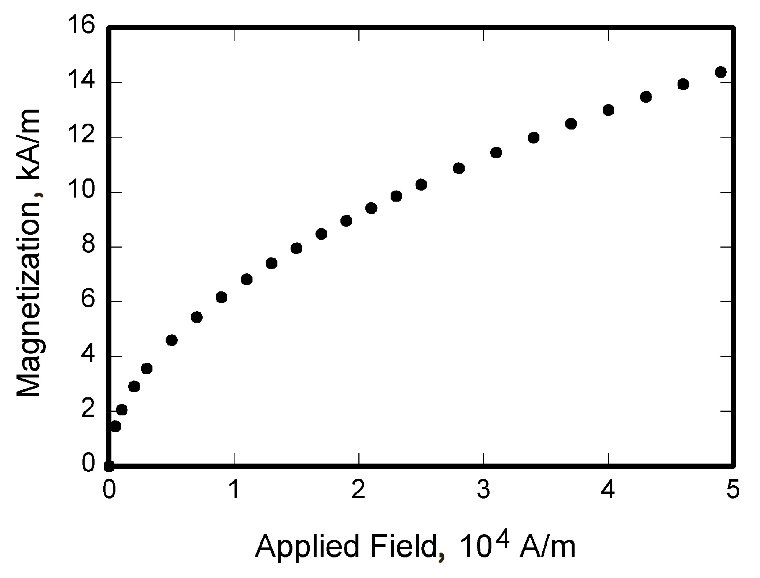
\includegraphics[width=.5\textwidth]{figures/graph.jpg}
  \caption{\quad \textbf{Magnetization as a function of applied fields.}}
  \label{fig:graph}
  \end{figure}

  \hspace{1em}
  
  \section{Measurement Results and Discussion}
  Present results with figures and tables. Analyze and interpret critically.

  \hspace{1em}

  \section{Conclusions}
  Summarize achievements, objectives met, lessons learned, future work.

  \hspace{1em}

  \bibliography{sample}

  \newpage
  \appendix
  \section{Appendix}
  Additional materials and data.

  \newpage
  \section{Supplementary}
\end{document}